% Created by tikzDevice version 0.6.2-92-0ad2792 on 2021-03-18 10:11:06
% !TEX encoding = UTF-8 Unicode
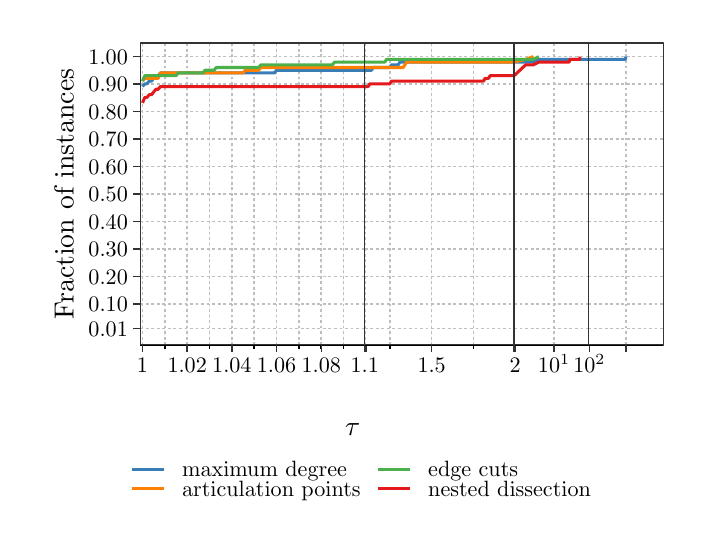
\begin{tikzpicture}[x=1pt,y=1pt]
\definecolor[named]{fillColor}{rgb}{1.00,1.00,1.00}
\path[use as bounding box,fill=fillColor,fill opacity=0.00] (0,0) rectangle (234.87,180.60);
\begin{scope}
\path[clip] (  0.00,  0.00) rectangle (234.87,180.60);
\definecolor[named]{drawColor}{rgb}{0.00,0.00,0.00}

\path[draw=drawColor,line width= 0.2pt,line join=round] ( 40.69, 65.91) --
	( 40.69,175.10);
\end{scope}
\begin{scope}
\path[clip] (  0.00,  0.00) rectangle (234.87,180.60);
\definecolor[named]{drawColor}{rgb}{0.00,0.00,0.00}

\node[text=drawColor,anchor=base east,inner sep=0pt, outer sep=0pt, scale=  0.80] at ( 36.19, 69.11) {0.01};

\node[text=drawColor,anchor=base east,inner sep=0pt, outer sep=0pt, scale=  0.80] at ( 36.19, 78.04) {0.10};

\node[text=drawColor,anchor=base east,inner sep=0pt, outer sep=0pt, scale=  0.80] at ( 36.19, 87.97) {0.20};

\node[text=drawColor,anchor=base east,inner sep=0pt, outer sep=0pt, scale=  0.80] at ( 36.19, 97.90) {0.30};

\node[text=drawColor,anchor=base east,inner sep=0pt, outer sep=0pt, scale=  0.80] at ( 36.19,107.82) {0.40};

\node[text=drawColor,anchor=base east,inner sep=0pt, outer sep=0pt, scale=  0.80] at ( 36.19,117.75) {0.50};

\node[text=drawColor,anchor=base east,inner sep=0pt, outer sep=0pt, scale=  0.80] at ( 36.19,127.68) {0.60};

\node[text=drawColor,anchor=base east,inner sep=0pt, outer sep=0pt, scale=  0.80] at ( 36.19,137.60) {0.70};

\node[text=drawColor,anchor=base east,inner sep=0pt, outer sep=0pt, scale=  0.80] at ( 36.19,147.53) {0.80};

\node[text=drawColor,anchor=base east,inner sep=0pt, outer sep=0pt, scale=  0.80] at ( 36.19,157.46) {0.90};

\node[text=drawColor,anchor=base east,inner sep=0pt, outer sep=0pt, scale=  0.80] at ( 36.19,167.38) {1.00};
\end{scope}
\begin{scope}
\path[clip] (  0.00,  0.00) rectangle (234.87,180.60);
\definecolor[named]{drawColor}{rgb}{0.20,0.20,0.20}

\path[draw=drawColor,line width= 0.5pt,line join=round] ( 38.19, 71.86) --
	( 40.69, 71.86);

\path[draw=drawColor,line width= 0.5pt,line join=round] ( 38.19, 80.80) --
	( 40.69, 80.80);

\path[draw=drawColor,line width= 0.5pt,line join=round] ( 38.19, 90.72) --
	( 40.69, 90.72);

\path[draw=drawColor,line width= 0.5pt,line join=round] ( 38.19,100.65) --
	( 40.69,100.65);

\path[draw=drawColor,line width= 0.5pt,line join=round] ( 38.19,110.58) --
	( 40.69,110.58);

\path[draw=drawColor,line width= 0.5pt,line join=round] ( 38.19,120.50) --
	( 40.69,120.50);

\path[draw=drawColor,line width= 0.5pt,line join=round] ( 38.19,130.43) --
	( 40.69,130.43);

\path[draw=drawColor,line width= 0.5pt,line join=round] ( 38.19,140.36) --
	( 40.69,140.36);

\path[draw=drawColor,line width= 0.5pt,line join=round] ( 38.19,150.29) --
	( 40.69,150.29);

\path[draw=drawColor,line width= 0.5pt,line join=round] ( 38.19,160.21) --
	( 40.69,160.21);

\path[draw=drawColor,line width= 0.5pt,line join=round] ( 38.19,170.14) --
	( 40.69,170.14);
\end{scope}
\begin{scope}
\path[clip] (  0.00,  0.00) rectangle (234.87,180.60);
\definecolor[named]{drawColor}{rgb}{0.00,0.00,0.00}

\node[text=drawColor,rotate= 90.00,anchor=base,inner sep=0pt, outer sep=0pt, scale=  1.00] at ( 16.56,120.50) {Fraction of instances};
\end{scope}
\begin{scope}
\path[clip] (  0.00,  0.00) rectangle (234.87,180.60);
\definecolor[named]{drawColor}{rgb}{0.00,0.00,0.00}

\path[draw=drawColor,line width= 0.2pt,line join=round] (121.82, 65.91) --
	(121.82,175.10);
\end{scope}
\begin{scope}
\path[clip] (  0.00,  0.00) rectangle (234.87,180.60);
\definecolor[named]{drawColor}{rgb}{0.20,0.20,0.20}

\path[draw=drawColor,line width= 0.5pt,line join=round] (119.32, 71.86) --
	(121.82, 71.86);

\path[draw=drawColor,line width= 0.5pt,line join=round] (119.32, 80.80) --
	(121.82, 80.80);

\path[draw=drawColor,line width= 0.5pt,line join=round] (119.32, 90.72) --
	(121.82, 90.72);

\path[draw=drawColor,line width= 0.5pt,line join=round] (119.32,100.65) --
	(121.82,100.65);

\path[draw=drawColor,line width= 0.5pt,line join=round] (119.32,110.58) --
	(121.82,110.58);

\path[draw=drawColor,line width= 0.5pt,line join=round] (119.32,120.50) --
	(121.82,120.50);

\path[draw=drawColor,line width= 0.5pt,line join=round] (119.32,130.43) --
	(121.82,130.43);

\path[draw=drawColor,line width= 0.5pt,line join=round] (119.32,140.36) --
	(121.82,140.36);

\path[draw=drawColor,line width= 0.5pt,line join=round] (119.32,150.29) --
	(121.82,150.29);

\path[draw=drawColor,line width= 0.5pt,line join=round] (119.32,160.21) --
	(121.82,160.21);

\path[draw=drawColor,line width= 0.5pt,line join=round] (119.32,170.14) --
	(121.82,170.14);
\end{scope}
\begin{scope}
\path[clip] (  0.00,  0.00) rectangle (234.87,180.60);
\definecolor[named]{drawColor}{rgb}{0.00,0.00,0.00}

\path[draw=drawColor,line width= 0.2pt,line join=round] (175.78, 65.91) --
	(175.78,175.10);
\end{scope}
\begin{scope}
\path[clip] (  0.00,  0.00) rectangle (234.87,180.60);
\definecolor[named]{drawColor}{rgb}{0.20,0.20,0.20}

\path[draw=drawColor,line width= 0.5pt,line join=round] (173.28, 71.86) --
	(175.78, 71.86);

\path[draw=drawColor,line width= 0.5pt,line join=round] (173.28, 80.80) --
	(175.78, 80.80);

\path[draw=drawColor,line width= 0.5pt,line join=round] (173.28, 90.72) --
	(175.78, 90.72);

\path[draw=drawColor,line width= 0.5pt,line join=round] (173.28,100.65) --
	(175.78,100.65);

\path[draw=drawColor,line width= 0.5pt,line join=round] (173.28,110.58) --
	(175.78,110.58);

\path[draw=drawColor,line width= 0.5pt,line join=round] (173.28,120.50) --
	(175.78,120.50);

\path[draw=drawColor,line width= 0.5pt,line join=round] (173.28,130.43) --
	(175.78,130.43);

\path[draw=drawColor,line width= 0.5pt,line join=round] (173.28,140.36) --
	(175.78,140.36);

\path[draw=drawColor,line width= 0.5pt,line join=round] (173.28,150.29) --
	(175.78,150.29);

\path[draw=drawColor,line width= 0.5pt,line join=round] (173.28,160.21) --
	(175.78,160.21);

\path[draw=drawColor,line width= 0.5pt,line join=round] (173.28,170.14) --
	(175.78,170.14);
\end{scope}
\begin{scope}
\path[clip] (  0.00,  0.00) rectangle (234.87,180.60);
\definecolor[named]{drawColor}{rgb}{0.00,0.00,0.00}

\path[draw=drawColor,line width= 0.2pt,line join=round] (202.55, 65.91) --
	(202.55,175.10);
\end{scope}
\begin{scope}
\path[clip] (  0.00,  0.00) rectangle (234.87,180.60);
\definecolor[named]{drawColor}{rgb}{0.20,0.20,0.20}

\path[draw=drawColor,line width= 0.5pt,line join=round] (200.05, 71.86) --
	(202.55, 71.86);

\path[draw=drawColor,line width= 0.5pt,line join=round] (200.05, 80.80) --
	(202.55, 80.80);

\path[draw=drawColor,line width= 0.5pt,line join=round] (200.05, 90.72) --
	(202.55, 90.72);

\path[draw=drawColor,line width= 0.5pt,line join=round] (200.05,100.65) --
	(202.55,100.65);

\path[draw=drawColor,line width= 0.5pt,line join=round] (200.05,110.58) --
	(202.55,110.58);

\path[draw=drawColor,line width= 0.5pt,line join=round] (200.05,120.50) --
	(202.55,120.50);

\path[draw=drawColor,line width= 0.5pt,line join=round] (200.05,130.43) --
	(202.55,130.43);

\path[draw=drawColor,line width= 0.5pt,line join=round] (200.05,140.36) --
	(202.55,140.36);

\path[draw=drawColor,line width= 0.5pt,line join=round] (200.05,150.29) --
	(202.55,150.29);

\path[draw=drawColor,line width= 0.5pt,line join=round] (200.05,160.21) --
	(202.55,160.21);

\path[draw=drawColor,line width= 0.5pt,line join=round] (200.05,170.14) --
	(202.55,170.14);
\end{scope}
\begin{scope}
\path[clip] (  0.00,  0.00) rectangle (234.87,180.60);
\definecolor[named]{fillColor}{rgb}{1.00,1.00,1.00}

\path[fill=fillColor] ( 40.69, 65.91) rectangle (122.22,175.10);
\definecolor[named]{drawColor}{rgb}{0.75,0.75,0.75}

\path[draw=drawColor,line width= 0.6pt,dash pattern=on 1pt off 1pt ,line join=round] ( 40.69, 71.86) --
	(122.22, 71.86);

\path[draw=drawColor,line width= 0.6pt,dash pattern=on 1pt off 1pt ,line join=round] ( 40.69, 80.80) --
	(122.22, 80.80);

\path[draw=drawColor,line width= 0.6pt,dash pattern=on 1pt off 1pt ,line join=round] ( 40.69, 90.72) --
	(122.22, 90.72);

\path[draw=drawColor,line width= 0.6pt,dash pattern=on 1pt off 1pt ,line join=round] ( 40.69,100.65) --
	(122.22,100.65);

\path[draw=drawColor,line width= 0.6pt,dash pattern=on 1pt off 1pt ,line join=round] ( 40.69,110.58) --
	(122.22,110.58);

\path[draw=drawColor,line width= 0.6pt,dash pattern=on 1pt off 1pt ,line join=round] ( 40.69,120.50) --
	(122.22,120.50);

\path[draw=drawColor,line width= 0.6pt,dash pattern=on 1pt off 1pt ,line join=round] ( 40.69,130.43) --
	(122.22,130.43);

\path[draw=drawColor,line width= 0.6pt,dash pattern=on 1pt off 1pt ,line join=round] ( 40.69,140.36) --
	(122.22,140.36);

\path[draw=drawColor,line width= 0.6pt,dash pattern=on 1pt off 1pt ,line join=round] ( 40.69,150.29) --
	(122.22,150.29);

\path[draw=drawColor,line width= 0.6pt,dash pattern=on 1pt off 1pt ,line join=round] ( 40.69,160.21) --
	(122.22,160.21);

\path[draw=drawColor,line width= 0.6pt,dash pattern=on 1pt off 1pt ,line join=round] ( 40.69,170.14) --
	(122.22,170.14);

\path[draw=drawColor,line width= 0.6pt,dash pattern=on 1pt off 1pt ,line join=round] ( 41.50, 65.91) --
	( 41.50,175.10);

\path[draw=drawColor,line width= 0.6pt,dash pattern=on 1pt off 1pt ,line join=round] ( 57.64, 65.91) --
	( 57.64,175.10);

\path[draw=drawColor,line width= 0.6pt,dash pattern=on 1pt off 1pt ,line join=round] ( 73.79, 65.91) --
	( 73.79,175.10);

\path[draw=drawColor,line width= 0.6pt,dash pattern=on 1pt off 1pt ,line join=round] ( 89.93, 65.91) --
	( 89.93,175.10);

\path[draw=drawColor,line width= 0.6pt,dash pattern=on 1pt off 1pt ,line join=round] (106.08, 65.91) --
	(106.08,175.10);

\path[draw=drawColor,line width= 0.6pt,dash pattern=on 1pt off 1pt ,line join=round] (122.22, 65.91) --
	(122.22,175.10);
\definecolor[named]{drawColor}{rgb}{0.00,0.00,0.00}
\definecolor[named]{fillColor}{rgb}{0.00,0.00,0.00}

\path[draw=drawColor,line width= 0.6pt,line join=round,fill=fillColor] ( 49.57, 64.42) -- ( 49.57, 65.91);

\path[draw=drawColor,line width= 0.6pt,line join=round,fill=fillColor] ( 57.64, 64.42) -- ( 57.64, 65.91);

\path[draw=drawColor,line width= 0.6pt,line join=round,fill=fillColor] ( 65.72, 64.42) -- ( 65.72, 65.91);

\path[draw=drawColor,line width= 0.6pt,line join=round,fill=fillColor] ( 73.79, 64.42) -- ( 73.79, 65.91);

\path[draw=drawColor,line width= 0.6pt,line join=round,fill=fillColor] ( 81.86, 64.42) -- ( 81.86, 65.91);

\path[draw=drawColor,line width= 0.6pt,line join=round,fill=fillColor] ( 89.93, 64.42) -- ( 89.93, 65.91);

\path[draw=drawColor,line width= 0.6pt,line join=round,fill=fillColor] ( 98.00, 64.42) -- ( 98.00, 65.91);

\path[draw=drawColor,line width= 0.6pt,line join=round,fill=fillColor] (106.08, 64.42) -- (106.08, 65.91);

\path[draw=drawColor,line width= 0.6pt,line join=round,fill=fillColor] (114.15, 64.42) -- (114.15, 65.91);
\definecolor[named]{drawColor}{rgb}{0.75,0.75,0.75}
\definecolor[named]{fillColor}{rgb}{0.75,0.75,0.75}

\path[draw=drawColor,line width= 0.6pt,dash pattern=on 1pt off 1pt ,line join=round,fill=fillColor] ( 49.57, 65.91) -- ( 49.57,175.10);

\path[draw=drawColor,line width= 0.6pt,dash pattern=on 1pt off 1pt ,line join=round,fill=fillColor] ( 57.64, 65.91) -- ( 57.64,175.10);

\path[draw=drawColor,line width= 0.6pt,dash pattern=on 1pt off 1pt ,line join=round,fill=fillColor] ( 65.72, 65.91) -- ( 65.72,175.10);

\path[draw=drawColor,line width= 0.6pt,dash pattern=on 1pt off 1pt ,line join=round,fill=fillColor] ( 73.79, 65.91) -- ( 73.79,175.10);

\path[draw=drawColor,line width= 0.6pt,dash pattern=on 1pt off 1pt ,line join=round,fill=fillColor] ( 81.86, 65.91) -- ( 81.86,175.10);

\path[draw=drawColor,line width= 0.6pt,dash pattern=on 1pt off 1pt ,line join=round,fill=fillColor] ( 89.93, 65.91) -- ( 89.93,175.10);

\path[draw=drawColor,line width= 0.6pt,dash pattern=on 1pt off 1pt ,line join=round,fill=fillColor] ( 98.00, 65.91) -- ( 98.00,175.10);

\path[draw=drawColor,line width= 0.6pt,dash pattern=on 1pt off 1pt ,line join=round,fill=fillColor] (106.08, 65.91) -- (106.08,175.10);

\path[draw=drawColor,line width= 0.6pt,dash pattern=on 1pt off 1pt ,line join=round,fill=fillColor] (114.15, 65.91) -- (114.15,175.10);
\definecolor[named]{drawColor}{rgb}{0.22,0.49,0.72}

\path[draw=drawColor,line width= 1.1pt,line join=round] ( 41.50,159.33) --
	( 42.31,160.31) --
	( 43.11,160.31) --
	( 43.92,161.29) --
	( 44.73,161.29) --
	( 45.53,162.28) --
	( 46.34,163.26) --
	( 47.15,163.26) --
	( 47.96,164.24) --
	( 48.76,164.24) --
	( 49.57,164.24) --
	( 50.38,164.24) --
	( 51.18,164.24) --
	( 51.99,164.24) --
	( 52.80,164.24) --
	( 53.61,164.24) --
	( 54.41,164.24) --
	( 55.22,164.24) --
	( 56.03,164.24) --
	( 56.84,164.24) --
	( 57.64,164.24) --
	( 58.45,164.24) --
	( 59.26,164.24) --
	( 60.06,164.24) --
	( 60.87,164.24) --
	( 61.68,164.24) --
	( 62.49,164.24) --
	( 63.29,164.24) --
	( 64.10,164.24) --
	( 64.91,164.24) --
	( 65.72,164.24) --
	( 66.52,164.24) --
	( 67.33,164.24) --
	( 68.14,164.24) --
	( 68.94,164.24) --
	( 69.75,164.24) --
	( 70.56,164.24) --
	( 71.37,164.24) --
	( 72.17,164.24) --
	( 72.98,164.24) --
	( 73.79,164.24) --
	( 74.59,164.24) --
	( 75.40,164.24) --
	( 76.21,164.24) --
	( 77.02,164.24) --
	( 77.82,164.24) --
	( 78.63,164.24) --
	( 79.44,164.24) --
	( 80.25,164.24) --
	( 81.05,164.24) --
	( 81.86,164.24) --
	( 82.67,164.24) --
	( 83.47,164.24) --
	( 84.28,164.24) --
	( 85.09,164.24) --
	( 85.90,164.24) --
	( 86.70,164.24) --
	( 87.51,164.24) --
	( 88.32,164.24) --
	( 89.12,164.24) --
	( 89.93,165.22) --
	( 90.74,165.22) --
	( 91.55,165.22) --
	( 92.35,165.22) --
	( 93.16,165.22) --
	( 93.97,165.22) --
	( 94.78,165.22) --
	( 95.58,165.22) --
	( 96.39,165.22) --
	( 97.20,165.22) --
	( 98.00,165.22) --
	( 98.81,165.22) --
	( 99.62,165.22) --
	(100.43,165.22) --
	(101.23,165.22) --
	(102.04,165.22) --
	(102.85,165.22) --
	(103.66,165.22) --
	(104.46,165.22) --
	(105.27,165.22) --
	(106.08,165.22) --
	(106.88,165.22) --
	(107.69,165.22) --
	(108.50,165.22) --
	(109.31,165.22) --
	(110.11,165.22) --
	(110.92,165.22) --
	(111.73,165.22) --
	(112.53,165.22) --
	(113.34,165.22) --
	(114.15,165.22) --
	(114.96,165.22) --
	(115.76,165.22) --
	(116.57,165.22) --
	(117.38,165.22) --
	(118.19,165.22) --
	(118.99,165.22) --
	(119.80,165.22) --
	(120.61,165.22) --
	(121.41,165.22) --
	(122.22,165.22) --
	(122.22,165.22);
\definecolor[named]{drawColor}{rgb}{1.00,0.50,0.00}

\path[draw=drawColor,line width= 1.1pt,line join=round] ( 41.50,161.29) --
	( 42.31,162.28) --
	( 43.11,162.28) --
	( 43.92,162.28) --
	( 44.73,162.28) --
	( 45.53,162.28) --
	( 46.34,162.28) --
	( 47.15,162.28) --
	( 47.96,164.24) --
	( 48.76,164.24) --
	( 49.57,164.24) --
	( 50.38,164.24) --
	( 51.18,164.24) --
	( 51.99,164.24) --
	( 52.80,164.24) --
	( 53.61,164.24) --
	( 54.41,164.24) --
	( 55.22,164.24) --
	( 56.03,164.24) --
	( 56.84,164.24) --
	( 57.64,164.24) --
	( 58.45,164.24) --
	( 59.26,164.24) --
	( 60.06,164.24) --
	( 60.87,164.24) --
	( 61.68,164.24) --
	( 62.49,164.24) --
	( 63.29,164.24) --
	( 64.10,164.24) --
	( 64.91,164.24) --
	( 65.72,164.24) --
	( 66.52,164.24) --
	( 67.33,164.24) --
	( 68.14,164.24) --
	( 68.94,164.24) --
	( 69.75,164.24) --
	( 70.56,164.24) --
	( 71.37,164.24) --
	( 72.17,164.24) --
	( 72.98,164.24) --
	( 73.79,164.24) --
	( 74.59,164.24) --
	( 75.40,164.24) --
	( 76.21,164.24) --
	( 77.02,164.24) --
	( 77.82,164.24) --
	( 78.63,165.22) --
	( 79.44,165.22) --
	( 80.25,165.22) --
	( 81.05,165.22) --
	( 81.86,165.22) --
	( 82.67,165.22) --
	( 83.47,165.22) --
	( 84.28,166.21) --
	( 85.09,166.21) --
	( 85.90,166.21) --
	( 86.70,166.21) --
	( 87.51,166.21) --
	( 88.32,166.21) --
	( 89.12,166.21) --
	( 89.93,166.21) --
	( 90.74,166.21) --
	( 91.55,166.21) --
	( 92.35,166.21) --
	( 93.16,166.21) --
	( 93.97,166.21) --
	( 94.78,166.21) --
	( 95.58,166.21) --
	( 96.39,166.21) --
	( 97.20,166.21) --
	( 98.00,166.21) --
	( 98.81,166.21) --
	( 99.62,166.21) --
	(100.43,166.21) --
	(101.23,166.21) --
	(102.04,166.21) --
	(102.85,166.21) --
	(103.66,166.21) --
	(104.46,166.21) --
	(105.27,166.21) --
	(106.08,166.21) --
	(106.88,166.21) --
	(107.69,166.21) --
	(108.50,166.21) --
	(109.31,166.21) --
	(110.11,166.21) --
	(110.92,166.21) --
	(111.73,166.21) --
	(112.53,166.21) --
	(113.34,166.21) --
	(114.15,166.21) --
	(114.96,166.21) --
	(115.76,166.21) --
	(116.57,166.21) --
	(117.38,166.21) --
	(118.19,166.21) --
	(118.99,166.21) --
	(119.80,166.21) --
	(120.61,166.21) --
	(121.41,166.21) --
	(122.22,166.21) --
	(122.22,166.21);
\definecolor[named]{drawColor}{rgb}{0.30,0.69,0.29}

\path[draw=drawColor,line width= 1.1pt,line join=round] ( 41.50,161.29) --
	( 42.31,163.26) --
	( 43.11,163.26) --
	( 43.92,163.26) --
	( 44.73,163.26) --
	( 45.53,163.26) --
	( 46.34,163.26) --
	( 47.15,163.26) --
	( 47.96,163.26) --
	( 48.76,163.26) --
	( 49.57,163.26) --
	( 50.38,163.26) --
	( 51.18,163.26) --
	( 51.99,163.26) --
	( 52.80,163.26) --
	( 53.61,163.26) --
	( 54.41,164.24) --
	( 55.22,164.24) --
	( 56.03,164.24) --
	( 56.84,164.24) --
	( 57.64,164.24) --
	( 58.45,164.24) --
	( 59.26,164.24) --
	( 60.06,164.24) --
	( 60.87,164.24) --
	( 61.68,164.24) --
	( 62.49,164.24) --
	( 63.29,164.24) --
	( 64.10,165.22) --
	( 64.91,165.22) --
	( 65.72,165.22) --
	( 66.52,165.22) --
	( 67.33,165.22) --
	( 68.14,166.21) --
	( 68.94,166.21) --
	( 69.75,166.21) --
	( 70.56,166.21) --
	( 71.37,166.21) --
	( 72.17,166.21) --
	( 72.98,166.21) --
	( 73.79,166.21) --
	( 74.59,166.21) --
	( 75.40,166.21) --
	( 76.21,166.21) --
	( 77.02,166.21) --
	( 77.82,166.21) --
	( 78.63,166.21) --
	( 79.44,166.21) --
	( 80.25,166.21) --
	( 81.05,166.21) --
	( 81.86,166.21) --
	( 82.67,166.21) --
	( 83.47,166.21) --
	( 84.28,167.19) --
	( 85.09,167.19) --
	( 85.90,167.19) --
	( 86.70,167.19) --
	( 87.51,167.19) --
	( 88.32,167.19) --
	( 89.12,167.19) --
	( 89.93,167.19) --
	( 90.74,167.19) --
	( 91.55,167.19) --
	( 92.35,167.19) --
	( 93.16,167.19) --
	( 93.97,167.19) --
	( 94.78,167.19) --
	( 95.58,167.19) --
	( 96.39,167.19) --
	( 97.20,167.19) --
	( 98.00,167.19) --
	( 98.81,167.19) --
	( 99.62,167.19) --
	(100.43,167.19) --
	(101.23,167.19) --
	(102.04,167.19) --
	(102.85,167.19) --
	(103.66,167.19) --
	(104.46,167.19) --
	(105.27,167.19) --
	(106.08,167.19) --
	(106.88,167.19) --
	(107.69,167.19) --
	(108.50,167.19) --
	(109.31,167.19) --
	(110.11,167.19) --
	(110.92,168.17) --
	(111.73,168.17) --
	(112.53,168.17) --
	(113.34,168.17) --
	(114.15,168.17) --
	(114.96,168.17) --
	(115.76,168.17) --
	(116.57,168.17) --
	(117.38,168.17) --
	(118.19,168.17) --
	(118.99,168.17) --
	(119.80,168.17) --
	(120.61,168.17) --
	(121.41,168.17) --
	(122.22,168.17) --
	(122.22,168.17);
\definecolor[named]{drawColor}{rgb}{0.89,0.10,0.11}

\path[draw=drawColor,line width= 1.1pt,line join=round] ( 41.50,153.43) --
	( 42.31,155.40) --
	( 43.11,155.40) --
	( 43.92,156.38) --
	( 44.73,156.38) --
	( 45.53,157.36) --
	( 46.34,158.34) --
	( 47.15,158.34) --
	( 47.96,159.33) --
	( 48.76,159.33) --
	( 49.57,159.33) --
	( 50.38,159.33) --
	( 51.18,159.33) --
	( 51.99,159.33) --
	( 52.80,159.33) --
	( 53.61,159.33) --
	( 54.41,159.33) --
	( 55.22,159.33) --
	( 56.03,159.33) --
	( 56.84,159.33) --
	( 57.64,159.33) --
	( 58.45,159.33) --
	( 59.26,159.33) --
	( 60.06,159.33) --
	( 60.87,159.33) --
	( 61.68,159.33) --
	( 62.49,159.33) --
	( 63.29,159.33) --
	( 64.10,159.33) --
	( 64.91,159.33) --
	( 65.72,159.33) --
	( 66.52,159.33) --
	( 67.33,159.33) --
	( 68.14,159.33) --
	( 68.94,159.33) --
	( 69.75,159.33) --
	( 70.56,159.33) --
	( 71.37,159.33) --
	( 72.17,159.33) --
	( 72.98,159.33) --
	( 73.79,159.33) --
	( 74.59,159.33) --
	( 75.40,159.33) --
	( 76.21,159.33) --
	( 77.02,159.33) --
	( 77.82,159.33) --
	( 78.63,159.33) --
	( 79.44,159.33) --
	( 80.25,159.33) --
	( 81.05,159.33) --
	( 81.86,159.33) --
	( 82.67,159.33) --
	( 83.47,159.33) --
	( 84.28,159.33) --
	( 85.09,159.33) --
	( 85.90,159.33) --
	( 86.70,159.33) --
	( 87.51,159.33) --
	( 88.32,159.33) --
	( 89.12,159.33) --
	( 89.93,159.33) --
	( 90.74,159.33) --
	( 91.55,159.33) --
	( 92.35,159.33) --
	( 93.16,159.33) --
	( 93.97,159.33) --
	( 94.78,159.33) --
	( 95.58,159.33) --
	( 96.39,159.33) --
	( 97.20,159.33) --
	( 98.00,159.33) --
	( 98.81,159.33) --
	( 99.62,159.33) --
	(100.43,159.33) --
	(101.23,159.33) --
	(102.04,159.33) --
	(102.85,159.33) --
	(103.66,159.33) --
	(104.46,159.33) --
	(105.27,159.33) --
	(106.08,159.33) --
	(106.88,159.33) --
	(107.69,159.33) --
	(108.50,159.33) --
	(109.31,159.33) --
	(110.11,159.33) --
	(110.92,159.33) --
	(111.73,159.33) --
	(112.53,159.33) --
	(113.34,159.33) --
	(114.15,159.33) --
	(114.96,159.33) --
	(115.76,159.33) --
	(116.57,159.33) --
	(117.38,159.33) --
	(118.19,159.33) --
	(118.99,159.33) --
	(119.80,159.33) --
	(120.61,159.33) --
	(121.41,159.33) --
	(122.22,159.33) --
	(122.22,159.33);
\definecolor[named]{drawColor}{rgb}{0.20,0.20,0.20}

\path[draw=drawColor,line width= 0.5pt,line join=round,line cap=round] ( 40.69, 65.91) rectangle (122.22,175.10);
\end{scope}
\begin{scope}
\path[clip] (  0.00,  0.00) rectangle (234.87,180.60);
\definecolor[named]{fillColor}{rgb}{1.00,1.00,1.00}

\path[fill=fillColor] (121.82, 65.91) rectangle (176.18,175.10);
\definecolor[named]{drawColor}{rgb}{0.75,0.75,0.75}

\path[draw=drawColor,line width= 0.6pt,dash pattern=on 1pt off 1pt ,line join=round] (121.82, 71.86) --
	(176.18, 71.86);

\path[draw=drawColor,line width= 0.6pt,dash pattern=on 1pt off 1pt ,line join=round] (121.82, 80.80) --
	(176.18, 80.80);

\path[draw=drawColor,line width= 0.6pt,dash pattern=on 1pt off 1pt ,line join=round] (121.82, 90.72) --
	(176.18, 90.72);

\path[draw=drawColor,line width= 0.6pt,dash pattern=on 1pt off 1pt ,line join=round] (121.82,100.65) --
	(176.18,100.65);

\path[draw=drawColor,line width= 0.6pt,dash pattern=on 1pt off 1pt ,line join=round] (121.82,110.58) --
	(176.18,110.58);

\path[draw=drawColor,line width= 0.6pt,dash pattern=on 1pt off 1pt ,line join=round] (121.82,120.50) --
	(176.18,120.50);

\path[draw=drawColor,line width= 0.6pt,dash pattern=on 1pt off 1pt ,line join=round] (121.82,130.43) --
	(176.18,130.43);

\path[draw=drawColor,line width= 0.6pt,dash pattern=on 1pt off 1pt ,line join=round] (121.82,140.36) --
	(176.18,140.36);

\path[draw=drawColor,line width= 0.6pt,dash pattern=on 1pt off 1pt ,line join=round] (121.82,150.29) --
	(176.18,150.29);

\path[draw=drawColor,line width= 0.6pt,dash pattern=on 1pt off 1pt ,line join=round] (121.82,160.21) --
	(176.18,160.21);

\path[draw=drawColor,line width= 0.6pt,dash pattern=on 1pt off 1pt ,line join=round] (121.82,170.14) --
	(176.18,170.14);

\path[draw=drawColor,line width= 0.6pt,dash pattern=on 1pt off 1pt ,line join=round] (121.82, 65.91) --
	(121.82,175.10);

\path[draw=drawColor,line width= 0.6pt,dash pattern=on 1pt off 1pt ,line join=round] (145.98, 65.91) --
	(145.98,175.10);

\path[draw=drawColor,line width= 0.6pt,dash pattern=on 1pt off 1pt ,line join=round] (176.18, 65.91) --
	(176.18,175.10);
\definecolor[named]{drawColor}{rgb}{0.00,0.00,0.00}
\definecolor[named]{fillColor}{rgb}{0.00,0.00,0.00}

\path[draw=drawColor,line width= 0.6pt,line join=round,fill=fillColor] (130.88, 64.42) -- (130.88, 65.91);

\path[draw=drawColor,line width= 0.6pt,line join=round,fill=fillColor] (145.98, 64.42) -- (145.98, 65.91);

\path[draw=drawColor,line width= 0.6pt,line join=round,fill=fillColor] (161.08, 64.42) -- (161.08, 65.91);
\definecolor[named]{drawColor}{rgb}{0.75,0.75,0.75}
\definecolor[named]{fillColor}{rgb}{0.75,0.75,0.75}

\path[draw=drawColor,line width= 0.6pt,dash pattern=on 1pt off 1pt ,line join=round,fill=fillColor] (130.88, 65.91) -- (130.88,175.10);

\path[draw=drawColor,line width= 0.6pt,dash pattern=on 1pt off 1pt ,line join=round,fill=fillColor] (145.98, 65.91) -- (145.98,175.10);

\path[draw=drawColor,line width= 0.6pt,dash pattern=on 1pt off 1pt ,line join=round,fill=fillColor] (161.08, 65.91) -- (161.08,175.10);
\definecolor[named]{drawColor}{rgb}{0.22,0.49,0.72}

\path[draw=drawColor,line width= 1.1pt,line join=round] (121.82,165.22) --
	(121.82,165.22) --
	(122.43,165.22) --
	(123.03,165.22) --
	(123.63,165.22) --
	(124.24,165.22) --
	(124.84,166.21) --
	(125.45,166.21) --
	(126.05,166.21) --
	(126.65,166.21) --
	(127.26,166.21) --
	(127.86,166.21) --
	(128.46,166.21) --
	(129.07,166.21) --
	(129.67,166.21) --
	(130.28,166.21) --
	(130.88,166.21) --
	(131.48,167.19) --
	(132.09,167.19) --
	(132.69,167.19) --
	(133.30,167.19) --
	(133.90,167.19) --
	(134.50,168.17) --
	(135.11,168.17) --
	(135.71,168.17) --
	(136.32,168.17) --
	(136.92,168.17) --
	(137.52,168.17) --
	(138.13,168.17) --
	(138.73,168.17) --
	(139.34,168.17) --
	(139.94,168.17) --
	(140.54,168.17) --
	(141.15,168.17) --
	(141.75,168.17) --
	(142.36,168.17) --
	(142.96,168.17) --
	(143.56,168.17) --
	(144.17,168.17) --
	(144.77,168.17) --
	(145.37,168.17) --
	(145.98,168.17) --
	(146.58,168.17) --
	(147.19,168.17) --
	(147.79,168.17) --
	(148.39,168.17) --
	(149.00,168.17) --
	(149.60,168.17) --
	(150.21,168.17) --
	(150.81,168.17) --
	(151.41,168.17) --
	(152.02,168.17) --
	(152.62,168.17) --
	(153.23,168.17) --
	(153.83,168.17) --
	(154.43,168.17) --
	(155.04,168.17) --
	(155.64,168.17) --
	(156.25,168.17) --
	(156.85,168.17) --
	(157.45,168.17) --
	(158.06,168.17) --
	(158.66,168.17) --
	(159.27,168.17) --
	(159.87,168.17) --
	(160.47,168.17) --
	(161.08,168.17) --
	(161.68,168.17) --
	(162.29,168.17) --
	(162.89,168.17) --
	(163.49,168.17) --
	(164.10,168.17) --
	(164.70,168.17) --
	(165.30,168.17) --
	(165.91,168.17) --
	(166.51,168.17) --
	(167.12,168.17) --
	(167.72,168.17) --
	(168.32,168.17) --
	(168.93,168.17) --
	(169.53,168.17) --
	(170.14,168.17) --
	(170.74,168.17) --
	(171.34,168.17) --
	(171.95,168.17) --
	(172.55,168.17) --
	(173.16,168.17) --
	(173.76,168.17) --
	(174.36,168.17) --
	(174.97,168.17) --
	(175.57,168.17) --
	(176.18,168.17) --
	(176.18,168.17);
\definecolor[named]{drawColor}{rgb}{1.00,0.50,0.00}

\path[draw=drawColor,line width= 1.1pt,line join=round] (121.82,166.21) --
	(121.82,166.21) --
	(122.43,166.21) --
	(123.03,166.21) --
	(123.63,166.21) --
	(124.24,166.21) --
	(124.84,166.21) --
	(125.45,166.21) --
	(126.05,166.21) --
	(126.65,166.21) --
	(127.26,166.21) --
	(127.86,166.21) --
	(128.46,166.21) --
	(129.07,166.21) --
	(129.67,166.21) --
	(130.28,166.21) --
	(130.88,166.21) --
	(131.48,166.21) --
	(132.09,166.21) --
	(132.69,166.21) --
	(133.30,166.21) --
	(133.90,166.21) --
	(134.50,166.21) --
	(135.11,166.21) --
	(135.71,166.21) --
	(136.32,167.19) --
	(136.92,168.17) --
	(137.52,168.17) --
	(138.13,168.17) --
	(138.73,168.17) --
	(139.34,168.17) --
	(139.94,168.17) --
	(140.54,168.17) --
	(141.15,168.17) --
	(141.75,168.17) --
	(142.36,168.17) --
	(142.96,168.17) --
	(143.56,168.17) --
	(144.17,168.17) --
	(144.77,168.17) --
	(145.37,168.17) --
	(145.98,168.17) --
	(146.58,168.17) --
	(147.19,168.17) --
	(147.79,168.17) --
	(148.39,168.17) --
	(149.00,168.17) --
	(149.60,168.17) --
	(150.21,168.17) --
	(150.81,168.17) --
	(151.41,168.17) --
	(152.02,168.17) --
	(152.62,168.17) --
	(153.23,168.17) --
	(153.83,168.17) --
	(154.43,168.17) --
	(155.04,168.17) --
	(155.64,168.17) --
	(156.25,168.17) --
	(156.85,168.17) --
	(157.45,168.17) --
	(158.06,168.17) --
	(158.66,168.17) --
	(159.27,168.17) --
	(159.87,168.17) --
	(160.47,168.17) --
	(161.08,168.17) --
	(161.68,168.17) --
	(162.29,168.17) --
	(162.89,168.17) --
	(163.49,168.17) --
	(164.10,168.17) --
	(164.70,168.17) --
	(165.30,168.17) --
	(165.91,168.17) --
	(166.51,168.17) --
	(167.12,168.17) --
	(167.72,168.17) --
	(168.32,168.17) --
	(168.93,168.17) --
	(169.53,168.17) --
	(170.14,168.17) --
	(170.74,168.17) --
	(171.34,168.17) --
	(171.95,168.17) --
	(172.55,168.17) --
	(173.16,168.17) --
	(173.76,168.17) --
	(174.36,168.17) --
	(174.97,168.17) --
	(175.57,168.17) --
	(176.18,168.17) --
	(176.18,168.17);
\definecolor[named]{drawColor}{rgb}{0.30,0.69,0.29}

\path[draw=drawColor,line width= 1.1pt,line join=round] (121.82,168.17) --
	(121.82,168.17) --
	(122.43,168.17) --
	(123.03,168.17) --
	(123.63,168.17) --
	(124.24,168.17) --
	(124.84,168.17) --
	(125.45,168.17) --
	(126.05,168.17) --
	(126.65,168.17) --
	(127.26,168.17) --
	(127.86,168.17) --
	(128.46,168.17) --
	(129.07,168.17) --
	(129.67,169.16) --
	(130.28,169.16) --
	(130.88,169.16) --
	(131.48,169.16) --
	(132.09,169.16) --
	(132.69,169.16) --
	(133.30,169.16) --
	(133.90,169.16) --
	(134.50,169.16) --
	(135.11,169.16) --
	(135.71,169.16) --
	(136.32,169.16) --
	(136.92,169.16) --
	(137.52,169.16) --
	(138.13,169.16) --
	(138.73,169.16) --
	(139.34,169.16) --
	(139.94,169.16) --
	(140.54,169.16) --
	(141.15,169.16) --
	(141.75,169.16) --
	(142.36,169.16) --
	(142.96,169.16) --
	(143.56,169.16) --
	(144.17,169.16) --
	(144.77,169.16) --
	(145.37,169.16) --
	(145.98,169.16) --
	(146.58,169.16) --
	(147.19,169.16) --
	(147.79,169.16) --
	(148.39,169.16) --
	(149.00,169.16) --
	(149.60,169.16) --
	(150.21,169.16) --
	(150.81,169.16) --
	(151.41,169.16) --
	(152.02,169.16) --
	(152.62,169.16) --
	(153.23,169.16) --
	(153.83,169.16) --
	(154.43,169.16) --
	(155.04,169.16) --
	(155.64,169.16) --
	(156.25,169.16) --
	(156.85,169.16) --
	(157.45,169.16) --
	(158.06,169.16) --
	(158.66,169.16) --
	(159.27,169.16) --
	(159.87,169.16) --
	(160.47,169.16) --
	(161.08,169.16) --
	(161.68,169.16) --
	(162.29,169.16) --
	(162.89,169.16) --
	(163.49,169.16) --
	(164.10,169.16) --
	(164.70,169.16) --
	(165.30,169.16) --
	(165.91,169.16) --
	(166.51,169.16) --
	(167.12,169.16) --
	(167.72,169.16) --
	(168.32,169.16) --
	(168.93,169.16) --
	(169.53,169.16) --
	(170.14,169.16) --
	(170.74,169.16) --
	(171.34,169.16) --
	(171.95,169.16) --
	(172.55,169.16) --
	(173.16,169.16) --
	(173.76,169.16) --
	(174.36,169.16) --
	(174.97,169.16) --
	(175.57,169.16) --
	(176.18,169.16) --
	(176.18,169.16);
\definecolor[named]{drawColor}{rgb}{0.89,0.10,0.11}

\path[draw=drawColor,line width= 1.1pt,line join=round] (121.82,159.33) --
	(121.82,159.33) --
	(122.43,159.33) --
	(123.03,159.33) --
	(123.63,160.31) --
	(124.24,160.31) --
	(124.84,160.31) --
	(125.45,160.31) --
	(126.05,160.31) --
	(126.65,160.31) --
	(127.26,160.31) --
	(127.86,160.31) --
	(128.46,160.31) --
	(129.07,160.31) --
	(129.67,160.31) --
	(130.28,160.31) --
	(130.88,160.31) --
	(131.48,161.29) --
	(132.09,161.29) --
	(132.69,161.29) --
	(133.30,161.29) --
	(133.90,161.29) --
	(134.50,161.29) --
	(135.11,161.29) --
	(135.71,161.29) --
	(136.32,161.29) --
	(136.92,161.29) --
	(137.52,161.29) --
	(138.13,161.29) --
	(138.73,161.29) --
	(139.34,161.29) --
	(139.94,161.29) --
	(140.54,161.29) --
	(141.15,161.29) --
	(141.75,161.29) --
	(142.36,161.29) --
	(142.96,161.29) --
	(143.56,161.29) --
	(144.17,161.29) --
	(144.77,161.29) --
	(145.37,161.29) --
	(145.98,161.29) --
	(146.58,161.29) --
	(147.19,161.29) --
	(147.79,161.29) --
	(148.39,161.29) --
	(149.00,161.29) --
	(149.60,161.29) --
	(150.21,161.29) --
	(150.81,161.29) --
	(151.41,161.29) --
	(152.02,161.29) --
	(152.62,161.29) --
	(153.23,161.29) --
	(153.83,161.29) --
	(154.43,161.29) --
	(155.04,161.29) --
	(155.64,161.29) --
	(156.25,161.29) --
	(156.85,161.29) --
	(157.45,161.29) --
	(158.06,161.29) --
	(158.66,161.29) --
	(159.27,161.29) --
	(159.87,161.29) --
	(160.47,161.29) --
	(161.08,161.29) --
	(161.68,161.29) --
	(162.29,161.29) --
	(162.89,161.29) --
	(163.49,161.29) --
	(164.10,161.29) --
	(164.70,161.29) --
	(165.30,162.28) --
	(165.91,162.28) --
	(166.51,162.28) --
	(167.12,163.26) --
	(167.72,163.26) --
	(168.32,163.26) --
	(168.93,163.26) --
	(169.53,163.26) --
	(170.14,163.26) --
	(170.74,163.26) --
	(171.34,163.26) --
	(171.95,163.26) --
	(172.55,163.26) --
	(173.16,163.26) --
	(173.76,163.26) --
	(174.36,163.26) --
	(174.97,163.26) --
	(175.57,163.26) --
	(176.18,163.26) --
	(176.18,163.26);
\definecolor[named]{drawColor}{rgb}{0.20,0.20,0.20}

\path[draw=drawColor,line width= 0.5pt,line join=round,line cap=round] (121.82, 65.91) rectangle (176.18,175.10);
\end{scope}
\begin{scope}
\path[clip] (  0.00,  0.00) rectangle (234.87,180.60);
\definecolor[named]{fillColor}{rgb}{1.00,1.00,1.00}

\path[fill=fillColor] (175.78, 65.91) rectangle (202.95,175.10);
\definecolor[named]{drawColor}{rgb}{0.75,0.75,0.75}

\path[draw=drawColor,line width= 0.6pt,dash pattern=on 1pt off 1pt ,line join=round] (175.78, 71.86) --
	(202.95, 71.86);

\path[draw=drawColor,line width= 0.6pt,dash pattern=on 1pt off 1pt ,line join=round] (175.78, 80.80) --
	(202.95, 80.80);

\path[draw=drawColor,line width= 0.6pt,dash pattern=on 1pt off 1pt ,line join=round] (175.78, 90.72) --
	(202.95, 90.72);

\path[draw=drawColor,line width= 0.6pt,dash pattern=on 1pt off 1pt ,line join=round] (175.78,100.65) --
	(202.95,100.65);

\path[draw=drawColor,line width= 0.6pt,dash pattern=on 1pt off 1pt ,line join=round] (175.78,110.58) --
	(202.95,110.58);

\path[draw=drawColor,line width= 0.6pt,dash pattern=on 1pt off 1pt ,line join=round] (175.78,120.50) --
	(202.95,120.50);

\path[draw=drawColor,line width= 0.6pt,dash pattern=on 1pt off 1pt ,line join=round] (175.78,130.43) --
	(202.95,130.43);

\path[draw=drawColor,line width= 0.6pt,dash pattern=on 1pt off 1pt ,line join=round] (175.78,140.36) --
	(202.95,140.36);

\path[draw=drawColor,line width= 0.6pt,dash pattern=on 1pt off 1pt ,line join=round] (175.78,150.29) --
	(202.95,150.29);

\path[draw=drawColor,line width= 0.6pt,dash pattern=on 1pt off 1pt ,line join=round] (175.78,160.21) --
	(202.95,160.21);

\path[draw=drawColor,line width= 0.6pt,dash pattern=on 1pt off 1pt ,line join=round] (175.78,170.14) --
	(202.95,170.14);

\path[draw=drawColor,line width= 0.6pt,dash pattern=on 1pt off 1pt ,line join=round] (175.78, 65.91) --
	(175.78,175.10);

\path[draw=drawColor,line width= 0.6pt,dash pattern=on 1pt off 1pt ,line join=round] (190.20, 65.91) --
	(190.20,175.10);

\path[draw=drawColor,line width= 0.6pt,dash pattern=on 1pt off 1pt ,line join=round] (202.95, 65.91) --
	(202.95,175.10);
\definecolor[named]{drawColor}{rgb}{0.22,0.49,0.72}

\path[draw=drawColor,line width= 1.1pt,line join=round] (175.78,168.17) --
	(175.78,168.17) --
	(179.97,168.17) --
	(182.71,168.17) --
	(184.69,169.16) --
	(186.24,169.16) --
	(187.49,169.16) --
	(188.53,169.16) --
	(189.43,169.16) --
	(190.20,169.16) --
	(190.89,169.16) --
	(191.50,169.16) --
	(192.05,169.16) --
	(192.55,169.16) --
	(193.01,169.16) --
	(193.43,169.16) --
	(193.82,169.16) --
	(194.18,169.16) --
	(194.52,169.16) --
	(194.84,169.16) --
	(195.14,169.16) --
	(195.42,169.16) --
	(195.68,169.16) --
	(195.93,169.16) --
	(196.17,169.16) --
	(196.39,169.16) --
	(196.61,169.16) --
	(196.81,169.16) --
	(197.01,169.16) --
	(197.20,169.16) --
	(197.38,169.16) --
	(197.55,169.16) --
	(197.72,169.16) --
	(197.88,169.16) --
	(198.04,169.16) --
	(198.19,169.16) --
	(198.33,169.16) --
	(198.47,169.16) --
	(198.60,169.16) --
	(198.74,169.16) --
	(198.86,169.16) --
	(198.99,169.16) --
	(199.10,169.16) --
	(199.22,169.16) --
	(199.33,169.16) --
	(199.44,169.16) --
	(199.55,169.16) --
	(199.65,169.16) --
	(199.75,169.16) --
	(199.85,169.16) --
	(199.95,169.16) --
	(200.04,169.16) --
	(200.13,169.16) --
	(200.22,169.16) --
	(200.31,169.16) --
	(200.40,169.16) --
	(200.48,169.16) --
	(200.56,169.16) --
	(200.64,169.16) --
	(200.72,169.16) --
	(200.80,169.16) --
	(200.87,169.16) --
	(200.95,169.16) --
	(201.02,169.16) --
	(201.09,169.16) --
	(201.16,169.16) --
	(201.23,169.16) --
	(201.29,169.16) --
	(201.36,169.16) --
	(201.42,169.16) --
	(201.49,169.16) --
	(201.55,169.16) --
	(201.61,169.16) --
	(201.67,169.16) --
	(201.73,169.16) --
	(201.79,169.16) --
	(201.85,169.16) --
	(201.90,169.16) --
	(201.96,169.16) --
	(202.01,169.16) --
	(202.07,169.16) --
	(202.12,169.16) --
	(202.17,169.16) --
	(202.22,169.16) --
	(202.27,169.16) --
	(202.32,169.16) --
	(202.37,169.16) --
	(202.42,169.16) --
	(202.47,169.16) --
	(202.52,169.16) --
	(202.56,169.16) --
	(202.61,169.16) --
	(202.65,169.16) --
	(202.70,169.16) --
	(202.74,169.16) --
	(202.78,169.16) --
	(202.83,169.16) --
	(202.87,169.16) --
	(202.91,169.16) --
	(202.95,169.16) --
	(202.95,169.16);
\definecolor[named]{drawColor}{rgb}{1.00,0.50,0.00}

\path[draw=drawColor,line width= 1.1pt,line join=round] (175.78,168.17) --
	(175.78,168.17) --
	(179.97,169.16) --
	(182.71,170.14);
\definecolor[named]{drawColor}{rgb}{0.30,0.69,0.29}

\path[draw=drawColor,line width= 1.1pt,line join=round] (175.78,169.16) --
	(175.78,169.16) --
	(179.97,169.16) --
	(182.71,169.16) --
	(184.69,170.14);
\definecolor[named]{drawColor}{rgb}{0.89,0.10,0.11}

\path[draw=drawColor,line width= 1.1pt,line join=round] (175.78,163.26) --
	(175.78,163.26) --
	(179.97,167.19) --
	(182.71,167.19) --
	(184.69,168.17) --
	(186.24,168.17) --
	(187.49,168.17) --
	(188.53,168.17) --
	(189.43,168.17) --
	(190.20,168.17) --
	(190.89,168.17) --
	(191.50,168.17) --
	(192.05,168.17) --
	(192.55,168.17) --
	(193.01,168.17) --
	(193.43,168.17) --
	(193.82,168.17) --
	(194.18,168.17) --
	(194.52,168.17) --
	(194.84,168.17) --
	(195.14,168.17) --
	(195.42,168.17) --
	(195.68,168.17) --
	(195.93,169.16) --
	(196.17,169.16) --
	(196.39,169.16) --
	(196.61,169.16) --
	(196.81,169.16) --
	(197.01,169.16) --
	(197.20,169.16) --
	(197.38,169.16) --
	(197.55,169.16) --
	(197.72,169.16) --
	(197.88,169.16) --
	(198.04,169.16) --
	(198.19,169.16) --
	(198.33,169.16) --
	(198.47,169.16) --
	(198.60,169.16) --
	(198.74,169.16) --
	(198.86,169.16) --
	(198.99,169.16) --
	(199.10,169.16) --
	(199.22,169.16) --
	(199.33,169.16) --
	(199.44,169.16) --
	(199.55,170.14);
\definecolor[named]{drawColor}{rgb}{0.20,0.20,0.20}

\path[draw=drawColor,line width= 0.5pt,line join=round,line cap=round] (175.78, 65.91) rectangle (202.95,175.10);
\end{scope}
\begin{scope}
\path[clip] (  0.00,  0.00) rectangle (234.87,180.60);
\definecolor[named]{fillColor}{rgb}{1.00,1.00,1.00}

\path[fill=fillColor] (202.55, 65.91) rectangle (229.73,175.10);
\definecolor[named]{drawColor}{rgb}{0.75,0.75,0.75}

\path[draw=drawColor,line width= 0.6pt,dash pattern=on 1pt off 1pt ,line join=round] (202.55, 71.86) --
	(229.73, 71.86);

\path[draw=drawColor,line width= 0.6pt,dash pattern=on 1pt off 1pt ,line join=round] (202.55, 80.80) --
	(229.73, 80.80);

\path[draw=drawColor,line width= 0.6pt,dash pattern=on 1pt off 1pt ,line join=round] (202.55, 90.72) --
	(229.73, 90.72);

\path[draw=drawColor,line width= 0.6pt,dash pattern=on 1pt off 1pt ,line join=round] (202.55,100.65) --
	(229.73,100.65);

\path[draw=drawColor,line width= 0.6pt,dash pattern=on 1pt off 1pt ,line join=round] (202.55,110.58) --
	(229.73,110.58);

\path[draw=drawColor,line width= 0.6pt,dash pattern=on 1pt off 1pt ,line join=round] (202.55,120.50) --
	(229.73,120.50);

\path[draw=drawColor,line width= 0.6pt,dash pattern=on 1pt off 1pt ,line join=round] (202.55,130.43) --
	(229.73,130.43);

\path[draw=drawColor,line width= 0.6pt,dash pattern=on 1pt off 1pt ,line join=round] (202.55,140.36) --
	(229.73,140.36);

\path[draw=drawColor,line width= 0.6pt,dash pattern=on 1pt off 1pt ,line join=round] (202.55,150.29) --
	(229.73,150.29);

\path[draw=drawColor,line width= 0.6pt,dash pattern=on 1pt off 1pt ,line join=round] (202.55,160.21) --
	(229.73,160.21);

\path[draw=drawColor,line width= 0.6pt,dash pattern=on 1pt off 1pt ,line join=round] (202.55,170.14) --
	(229.73,170.14);

\path[draw=drawColor,line width= 0.6pt,dash pattern=on 1pt off 1pt ,line join=round] (216.14, 65.91) --
	(216.14,175.10);
\definecolor[named]{drawColor}{rgb}{0.22,0.49,0.72}

\path[draw=drawColor,line width= 1.1pt,line join=round] (202.55,169.16) --
	(202.69,169.16) --
	(202.82,169.16) --
	(202.96,169.16) --
	(203.10,169.16) --
	(203.23,169.16) --
	(203.37,169.16) --
	(203.50,169.16) --
	(203.64,169.16) --
	(203.78,169.16) --
	(203.91,169.16) --
	(204.05,169.16) --
	(204.18,169.16) --
	(204.32,169.16) --
	(204.45,169.16) --
	(204.59,169.16) --
	(204.73,169.16) --
	(204.86,169.16) --
	(205.00,169.16) --
	(205.13,169.16) --
	(205.27,169.16) --
	(205.41,169.16) --
	(205.54,169.16) --
	(205.68,169.16) --
	(205.81,169.16) --
	(205.95,169.16) --
	(206.09,169.16) --
	(206.22,169.16) --
	(206.36,169.16) --
	(206.49,169.16) --
	(206.63,169.16) --
	(206.76,169.16) --
	(206.90,169.16) --
	(207.04,169.16) --
	(207.17,169.16) --
	(207.31,169.16) --
	(207.44,169.16) --
	(207.58,169.16) --
	(207.72,169.16) --
	(207.85,169.16) --
	(207.99,169.16) --
	(208.12,169.16) --
	(208.26,169.16) --
	(208.40,169.16) --
	(208.53,169.16) --
	(208.67,169.16) --
	(208.80,169.16) --
	(208.94,169.16) --
	(209.07,169.16) --
	(209.21,169.16) --
	(209.35,169.16) --
	(209.48,169.16) --
	(209.62,169.16) --
	(209.75,169.16) --
	(209.89,169.16) --
	(210.03,169.16) --
	(210.16,169.16) --
	(210.30,169.16) --
	(210.43,169.16) --
	(210.57,169.16) --
	(210.71,169.16) --
	(210.84,169.16) --
	(210.98,169.16) --
	(211.11,169.16) --
	(211.25,169.16) --
	(211.38,169.16) --
	(211.52,169.16) --
	(211.66,169.16) --
	(211.79,169.16) --
	(211.93,169.16) --
	(212.06,169.16) --
	(212.20,169.16) --
	(212.34,169.16) --
	(212.47,169.16) --
	(212.61,169.16) --
	(212.74,169.16) --
	(212.88,169.16) --
	(213.02,169.16) --
	(213.15,169.16) --
	(213.29,169.16) --
	(213.42,169.16) --
	(213.56,169.16) --
	(213.69,169.16) --
	(213.83,169.16) --
	(213.97,169.16) --
	(214.10,169.16) --
	(214.24,169.16) --
	(214.37,169.16) --
	(214.51,169.16) --
	(214.65,169.16) --
	(214.78,169.16) --
	(214.92,169.16) --
	(215.05,169.16) --
	(215.19,169.16) --
	(215.33,169.16) --
	(215.46,169.16) --
	(215.60,169.16) --
	(215.73,169.16) --
	(215.87,169.16) --
	(216.01,169.16) --
	(216.14,170.14);
\definecolor[named]{drawColor}{rgb}{0.20,0.20,0.20}

\path[draw=drawColor,line width= 0.5pt,line join=round,line cap=round] (202.55, 65.91) rectangle (229.73,175.10);
\end{scope}
\begin{scope}
\path[clip] (  0.00,  0.00) rectangle (234.87,180.60);
\definecolor[named]{drawColor}{rgb}{0.00,0.00,0.00}

\path[draw=drawColor,line width= 0.2pt,line join=round] ( 40.69, 65.91) --
	(122.22, 65.91);
\end{scope}
\begin{scope}
\path[clip] (  0.00,  0.00) rectangle (234.87,180.60);
\definecolor[named]{drawColor}{rgb}{0.20,0.20,0.20}

\path[draw=drawColor,line width= 0.5pt,line join=round] ( 41.50, 63.41) --
	( 41.50, 65.91);

\path[draw=drawColor,line width= 0.5pt,line join=round] ( 57.64, 63.41) --
	( 57.64, 65.91);

\path[draw=drawColor,line width= 0.5pt,line join=round] ( 73.79, 63.41) --
	( 73.79, 65.91);

\path[draw=drawColor,line width= 0.5pt,line join=round] ( 89.93, 63.41) --
	( 89.93, 65.91);

\path[draw=drawColor,line width= 0.5pt,line join=round] (106.08, 63.41) --
	(106.08, 65.91);

\path[draw=drawColor,line width= 0.5pt,line join=round] (122.22, 63.41) --
	(122.22, 65.91);
\end{scope}
\begin{scope}
\path[clip] (  0.00,  0.00) rectangle (234.87,180.60);
\definecolor[named]{drawColor}{rgb}{0.00,0.00,0.00}

\node[text=drawColor,anchor=base,inner sep=0pt, outer sep=0pt, scale=  0.80] at ( 41.50, 55.90) {1};

\node[text=drawColor,anchor=base,inner sep=0pt, outer sep=0pt, scale=  0.80] at ( 57.64, 55.90) {1.02};

\node[text=drawColor,anchor=base,inner sep=0pt, outer sep=0pt, scale=  0.80] at ( 73.79, 55.90) {1.04};

\node[text=drawColor,anchor=base,inner sep=0pt, outer sep=0pt, scale=  0.80] at ( 89.93, 55.90) {1.06};

\node[text=drawColor,anchor=base,inner sep=0pt, outer sep=0pt, scale=  0.80] at (106.08, 55.90) {1.08};
\end{scope}
\begin{scope}
\path[clip] (  0.00,  0.00) rectangle (234.87,180.60);
\definecolor[named]{drawColor}{rgb}{0.00,0.00,0.00}

\path[draw=drawColor,line width= 0.2pt,line join=round] (121.82, 65.91) --
	(176.18, 65.91);
\end{scope}
\begin{scope}
\path[clip] (  0.00,  0.00) rectangle (234.87,180.60);
\definecolor[named]{drawColor}{rgb}{0.20,0.20,0.20}

\path[draw=drawColor,line width= 0.5pt,line join=round] (121.82, 63.41) --
	(121.82, 65.91);

\path[draw=drawColor,line width= 0.5pt,line join=round] (145.98, 63.41) --
	(145.98, 65.91);

\path[draw=drawColor,line width= 0.5pt,line join=round] (176.18, 63.41) --
	(176.18, 65.91);
\end{scope}
\begin{scope}
\path[clip] (  0.00,  0.00) rectangle (234.87,180.60);
\definecolor[named]{drawColor}{rgb}{0.00,0.00,0.00}

\node[text=drawColor,anchor=base,inner sep=0pt, outer sep=0pt, scale=  0.80] at (121.82, 55.90) {1.1};

\node[text=drawColor,anchor=base,inner sep=0pt, outer sep=0pt, scale=  0.80] at (145.98, 55.90) {1.5};

\node[text=drawColor,anchor=base,inner sep=0pt, outer sep=0pt, scale=  0.80] at (176.18, 55.90) {2};
\end{scope}
\begin{scope}
\path[clip] (  0.00,  0.00) rectangle (234.87,180.60);
\definecolor[named]{drawColor}{rgb}{0.00,0.00,0.00}

\path[draw=drawColor,line width= 0.2pt,line join=round] (175.78, 65.91) --
	(202.95, 65.91);
\end{scope}
\begin{scope}
\path[clip] (  0.00,  0.00) rectangle (234.87,180.60);
\definecolor[named]{drawColor}{rgb}{0.20,0.20,0.20}

\path[draw=drawColor,line width= 0.5pt,line join=round] (175.78, 63.41) --
	(175.78, 65.91);

\path[draw=drawColor,line width= 0.5pt,line join=round] (190.20, 63.41) --
	(190.20, 65.91);

\path[draw=drawColor,line width= 0.5pt,line join=round] (202.95, 63.41) --
	(202.95, 65.91);
\end{scope}
\begin{scope}
\path[clip] (  0.00,  0.00) rectangle (234.87,180.60);
\definecolor[named]{drawColor}{rgb}{0.00,0.00,0.00}

\node[text=drawColor,anchor=base,inner sep=0pt, outer sep=0pt, scale=  0.80] at (190.20, 55.90) {$10^{1}$};

\node[text=drawColor,anchor=base,inner sep=0pt, outer sep=0pt, scale=  0.80] at (202.95, 55.90) {$10^{2}$};
\end{scope}
\begin{scope}
\path[clip] (  0.00,  0.00) rectangle (234.87,180.60);
\definecolor[named]{drawColor}{rgb}{0.00,0.00,0.00}

\path[draw=drawColor,line width= 0.2pt,line join=round] (202.55, 65.91) --
	(229.73, 65.91);
\end{scope}
\begin{scope}
\path[clip] (  0.00,  0.00) rectangle (234.87,180.60);
\definecolor[named]{drawColor}{rgb}{0.20,0.20,0.20}

\path[draw=drawColor,line width= 0.5pt,line join=round] (216.14, 63.41) --
	(216.14, 65.91);
\end{scope}
\begin{scope}
\path[clip] (  0.00,  0.00) rectangle (234.87,180.60);
\definecolor[named]{drawColor}{rgb}{0.00,0.00,0.00}

\node[text=drawColor,anchor=base,inner sep=0pt, outer sep=0pt, scale=  0.80] at (216.14, 55.90) {\ClockLogo};
\end{scope}
\begin{scope}
\path[clip] (  5.14, 30.10) rectangle (229.73, 43.01);
\definecolor[named]{drawColor}{rgb}{0.00,0.00,0.00}

\node[text=drawColor,anchor=base,inner sep=0pt, outer sep=0pt, scale=  1.00] at (117.44, 33.11) {$\tau$};
\end{scope}
\begin{scope}
\path[clip] (  0.00,  0.00) rectangle (234.87,180.60);
\definecolor[named]{drawColor}{rgb}{0.22,0.49,0.72}
\definecolor[named]{fillColor}{rgb}{0.22,0.49,0.72}

\path[draw=drawColor,line width= 1.1pt,line join=round,fill=fillColor] ( 37.79, 21.08) -- ( 49.35, 21.08);
\end{scope}
\begin{scope}
\path[clip] (  0.00,  0.00) rectangle (234.87,180.60);
\definecolor[named]{drawColor}{rgb}{1.00,0.50,0.00}
\definecolor[named]{fillColor}{rgb}{1.00,0.50,0.00}

\path[draw=drawColor,line width= 1.1pt,line join=round,fill=fillColor] ( 37.79, 14.02) -- ( 49.35, 14.02);
\end{scope}
\begin{scope}
\path[clip] (  0.00,  0.00) rectangle (234.87,180.60);
\definecolor[named]{drawColor}{rgb}{0.30,0.69,0.29}
\definecolor[named]{fillColor}{rgb}{0.30,0.69,0.29}

\path[draw=drawColor,line width= 1.1pt,line join=round,fill=fillColor] (126.74, 21.08) -- (138.30, 21.08);
\end{scope}
\begin{scope}
\path[clip] (  0.00,  0.00) rectangle (234.87,180.60);
\definecolor[named]{drawColor}{rgb}{0.89,0.10,0.11}
\definecolor[named]{fillColor}{rgb}{0.89,0.10,0.11}

\path[draw=drawColor,line width= 1.1pt,line join=round,fill=fillColor] (126.74, 14.02) -- (138.30, 14.02);
\end{scope}
\begin{scope}
\path[clip] (  0.00,  0.00) rectangle (234.87,180.60);
\definecolor[named]{drawColor}{rgb}{0.00,0.00,0.00}

\node[text=drawColor,anchor=base west,inner sep=0pt, outer sep=0pt, scale=  0.80] at ( 55.79, 18.33) {maximum degree};
\end{scope}
\begin{scope}
\path[clip] (  0.00,  0.00) rectangle (234.87,180.60);
\definecolor[named]{drawColor}{rgb}{0.00,0.00,0.00}

\node[text=drawColor,anchor=base west,inner sep=0pt, outer sep=0pt, scale=  0.80] at ( 55.79, 11.26) {articulation points};
\end{scope}
\begin{scope}
\path[clip] (  0.00,  0.00) rectangle (234.87,180.60);
\definecolor[named]{drawColor}{rgb}{0.00,0.00,0.00}

\node[text=drawColor,anchor=base west,inner sep=0pt, outer sep=0pt, scale=  0.80] at (144.74, 18.33) {edge cuts};
\end{scope}
\begin{scope}
\path[clip] (  0.00,  0.00) rectangle (234.87,180.60);
\definecolor[named]{drawColor}{rgb}{0.00,0.00,0.00}

\node[text=drawColor,anchor=base west,inner sep=0pt, outer sep=0pt, scale=  0.80] at (144.74, 11.26) {nested dissection};
\end{scope}
\end{tikzpicture}
